\chapter{Proposed Approach, Novelty \& Initial Experiment}

\section{Proposed Methodology (High-level Pipeline)}

Figure~\ref{fig:ProposeArchitecture} shows the overall high-level architecture of our proposed system. We adopt a multimodal input approach from SeeAct\cite{SeeAct}, with the Idea to combine the Action generation and grounding in same, where LMM handles the inference for grounding as well. Instead of passing the entire HTML DOM, we plan to use a Summarization before input to reduce the token input size while doing model inference. The agent outputs a structured plan with required values (action + target + value + HITL confidence + fallback confidence), which then we can use to validate the fallback or human-in-the-loop. on good confidence value we further can use action, target and value to execute that step using any environment controller tool (i.e. selenium).

\begin{figure}[h]
  \centering
  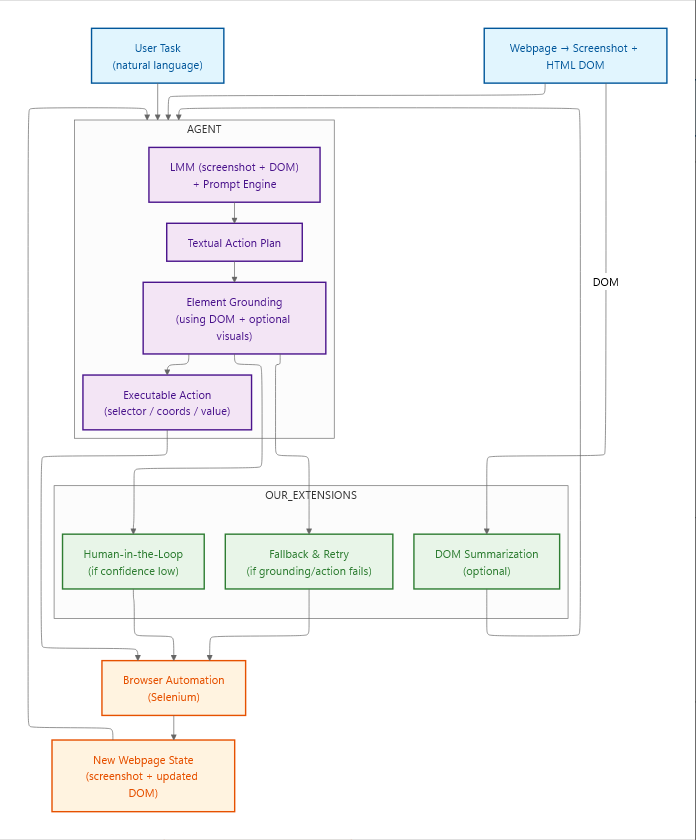
\includegraphics[width=0.6\textwidth]{Implementation Architecture.png}
  \caption{Proposed System Architecture: DOM summarizer, fallback and HITL.}
  \label{fig:ProposeArchitecture}
\end{figure}


\section{Novel Contributions (Experimental)}

\subsection{DOM Summarization for Token Efficiency}

Modern websites' webpages contain large HTML, noisy values, complex structure, and hidden elements, which Large Foundation Models do not access directly as input due to input size limits.
By summarising the HTML values and extracting only relevant elements and removing the unnecessary values, we can ask model to infer the value directly. This allows us to run automation on complex websites as well, without losing higher context for the grounding. 

\subsection{Zero-Shot and Few-Shot Prompting Strategy}
Rather than only fine-tuning heavy models on large datasets, we explore the prompt engineering techniques such as zero-shot mode (give input and expect output directly) and few-shot (input contains a few examples or an input-output pair, using which the model infer better) mode as well. This approach allows rapid experimentation with minimal additional data — useful under resource constraints and useful for evaluating generalization.

\subsection{Fallback + Human-in-the-Loop Mechanism}
We incorporate a fallback + HITL option because correct element grounding is known to be challenging. If the model produces a low-confidence action or an ambiguous target, the system either re-prompts the model or requests human approval before acting.  
This hybrid architecture strikes a compromise between automation efficiency, dependability, and safety. it is particularly helpful in delicate GUI tasks or early-stage experiments.

\section{Initial Experiment Setup}

\subsection{Environment, Tools, Model Used}
For our initial proof-of-concept, we configured the following environment:  
\begin{itemize}
  \item \textbf{Tools:} We use Python programming along with PyTorch to use models, a GPU, and interaction with the model.
  \item \textbf{Model:} Qwen2-VL-2B (lightweight multimodal model) , Qwen2 models are easily available from Hugging Face and come up with the desired size.
  \item \textbf{Browser Automation:} Selenium to programmatically trigger UI events. It provides an environment for experimentation.
  \item \textbf{Programming Language / Framework:} Python, with JSON parsing for model output and custom scripts for preprocessing, Summarization, grounding, and execution
\end{itemize}

\subsection{Data Loading \& Preprocessing}
We used a sample from the multimodal GUI dataset containing:  
\begin{itemize}
  \item The \emph{webpage screenshot} (visual snapshot)  
  \item The \emph{full HTML DOM} source corresponding to the screenshot  
  \item A natural-language task instruction  
\end{itemize}
In the preprocessing step:  
\begin{itemize}
  \item A single step data is loaded from parquet files. and simple sample pre-processing applied.
  \item (For baseline) instead of summarization of full dom we apply trimming on DOM, although it is not feasible technique, but we can test initial experiments.
  \item The inputs (screenshot + DOM + task) are packaged to form the model prompt  
\end{itemize}

\section{Inference Pipeline \& Prompting Details}
We enforce a strict JSON output schema from the model to ensure machine-parsable results.  
The prompt asks the agent to output exactly one JSON object with keys: \texttt{action}, \texttt{target}, \texttt{value}, \texttt{confidence}.  
Here, actions are {"click", "type", "scroll", "noop"}, target is either a CSS selector or coords, and value is a string or null.  
This structured output simplifies grounding, parsing, and subsequent browser execution or fallback decision.

\section{Initial Results and Observations}
On our first sample run:  
\begin{itemize}
  \item The model predicted \texttt{action = "click"} with a high \texttt{confidence = 0.99}.  Where, actuall ground truth action was click, which align with output.
  \item The predicted \texttt{target} was a CSS selector string — however, this selector did not correspond to any valid element in the DOM (i.e. grounding failed / hallucination occurred).  
  \item The \texttt{value} field was \texttt{null}, which was acceptable for the task.  
\end{itemize}

\noindent \textbf{These results show two important facts:}
\begin{enumerate}
    \item The pipeline (data loading → multimodal prompt → structured output → parsing) works end-to-end.  
    \item Grounding remains a serious challenge, Although we have used trimmed DOM and screenshot and high-confidence prediction clearly showcase the need for DOM summarization and fallback/HITL mechanisms.
\end{enumerate}
This early experiment confirms feasibility of the system design, while also shows core limitations to address in future work.

\bigskip  
\noindent In the next phases, we plan to 1. implement the DOM summarization module, 2. perform evaluation across multiple metrics, 3. add implement fallback and HITL logic, and 4. collect metrics for action, target, and value accuracy at scale.  
